\chapter{Fundamentação Teórica}\label{chapter:fundamentacao}
Neste capítulo, pretende-se oferecer ao leitor uma visão geral das principais áreas nas quais esse trabalho está fundamentado. Mais especificamente, uma explanação sobre o~\ac{dp}, seus sinais motores, os estágios da doença, o uso da cinemetria como ferramenta para medição dos parâmetros cinemáticos do movimento humano, e a~\ac{svm} como classificador de dados para a identificação dos padrões presentes em um conjunto de dados.


\section{Doença de Parkinson}\label{section:doenca_parkinson}
O termo Parkinsonismo é genérico e designa uma série de doenças com causas diferentes, que têm em comum a presença de sinais frequentemente encontrados no~\ac{dp}. Esta doença é uma das muitas formas de parkinsonismo, correspondendo a cerca de 75$\%$ dos casos. Os sinais associados ao~\ac{dp}~\cite{protpar010} são causados pela degeneração dos neurônios dopaminérgicos presentes na substância negra. O~\ac{dp} é mais comum em idosos, porém existem casos precoces de início da doença em indivíduos antes dos 40 anos ou até mesmo abaixo dos 21~\cite{menezes2003}. A incidência da doença é estimada de 100 a 200 casos por 100.000 habitantes e, com o avanço da idade populacional, o contingente de pessoas diagnosticadas com ~\ac{dp} tende a aumentar.

O~\ac{dp} é uma doença progressiva e incapacitante e, após os 10 anos de tratamento, o custo operacional, o impacto social e financeiro aumentam vertiginosamente. Estima-se que o custo anual mundial com medicamentos antiparkinsonianos esteja em torno de 11 bilhões de dólares, tornando-se de 3 a 4 vezes mais caro nas fases avançadas da doença~\cite{protpar010}. Outro fator crucial para a escolha do~\ac{dp} como objeto de estudo é a variação dos sinais motores ao longo do dia em virtude da resposta ao tratamento medicamentoso. Portanto, a abordagem de monitorar os sinais, em diferentes momentos do dia, permite um melhor gerenciamento da doença e, como consequência, uma melhora na qualidade de vida dessa população.


%TODO verificar a regencia do verbo acarretar: se for indireto mantém o em; caso contrário remove-o
Atualmente, o levodopa é o tratamento medicamentoso mais utilizado para o tratamento de redução dos sinais do~\ac{dp}. Porém, sua efetividade é reduzida ao longo do tempo, o que requer um aumento progressivo das dosagens ou o uso de outros tratamentos associados. Isso acarreta em um gerenciamento complexo entre drogas e seus respectivos efeitos colaterais. Portanto, ao buscar prolongar a qualidade de vida dos pacientes com o uso deste tratamento, é recomendável um gerenciamento medicamentoso com uma dosagem mínima~\cite{national2006parkinson}, para reduzir os sinais motores e prolongar a qualidade de vida do paciente. Como o gerenciamento medicamentoso é de responsabilidade do neurologista, este o faz de acordo com as visitas clínicas dos pacientes, quando estes ou seus cuidadores fazem relatos sobre o progresso do tratamento. Contudo, esta avaliação clínica é realizada de forma esporádica e subjetiva~\cite{protpar010,quantitativeparkinson2011}. Dessa maneira, é necessário uma quantificação destes sinais 
para um tratamento mais adequado e preciso. 

Com o surgimento do tratamento para o \ac{dp} é possível manter uma mobilidade funcional durante anos, além de aumentar a expectativa de vida dos pacientes tratados~\cite{rodrigues2006}. Os fármacos do grupo dos antiparkinsonianos, como a levodopa, permitem restaurar a atividade dopaminérgica que se encontra reduzida; dessa maneira, as drogas aliviam os sinais característicos da doença. Entretanto, devido aos efeitos colaterais frequentes induzidos pelos fármacos, é preciso iniciar o tratamento com esses medicamentos somente quando os sinais estiverem prejudicando o desempenho profissional ou as atividades diárias do paciente~\cite{rodrigues2006}. A natureza progressiva do~\ac{dp} e suas manifestações clínicas (motoras e não motoras) estão associadas a efeitos colaterais precoces e tardios da intervenção terapêutica, o que torna o tratamento da doença bastante complexo~\cite{protpar010}. Estima-se que a taxa de morte dos neurônios dopaminérgicos da substância negra situa-se ao redor de 10$\%$ ao ano~\cite{national2006parkinson}. Consequentemente, com o passar do tempo, a sintomatologia parkinsoniana tende a evoluir, o que aumenta a necessidade de uma maior dosagem medicamentosa, pois a resposta aos medicamentos decresce com o progresso da doença~\cite{protpar010}.

 
\subsection{Diagnóstico}
Os sinais mais característicos do ~\ac{dp} e que são frequentemente usados para diagnosticar a doença são~\cite{rowlandtratado}: tremor em repouso (que diminui durante movimentos voluntários); bradicinesia (lentidão e escassez de movimentos, além de dificuldade na marcha); rigidez muscular (aumento da resistência ao movimento passivo dos membros); e perda de reflexos posturais, que leva à alteração da marcha e aumenta a ocorrência de queda~\cite{rodrigues2006,tolosa06}. 

A evolução da doença, a gravidade e a progressão dos sinais variam de um paciente para outro. Atualmente, não existe teste diagnóstico estabelecido para a doença, e os estudos comprovam dificuldade na diferenciação clínica entre o~\ac{dp} e outras formas de parkinsonismo. A maioria dos neurologistas concorda que o diagnóstico do~\ac{dp} requer a identificação de alguma combinação de sinais motores cardinais, como: tremor de repouso, bradicinesia, rigidez tipo roda denteada e alterações posturais. No entanto, uma classificação clínica padrão ainda não foi obtida~\cite{protpar010}. Além do mais, um diagnóstico auxiliar importante é a resposta dos pacientes aos medicamentos antiparkinsonianos, tal como a levodopa~\cite{protpar010}. Os protocolos clínicos~\cite{protpar010,national2006parkinson} sugerem que o diagnóstico do~\ac{dp} está diretamente relacionado à resposta satisfatória ao levodopa. No entanto, uma resposta satisfatória à levodopa não confirma o diagnóstico do~\ac{dp}~\cite{rowlandtratado}, porque 
existem muitos casos de parkinsonismo sintomáticos e muitas formas de síndromes de Parkinson, que, em seus estágios iniciais, respondem bem ao levodopa. 

Atualmente, os critérios estabelecidos pelo Banco de Cérebros da Sociedade de Parkinson do Reino Unido~\cite{national2006parkinson} são os mais utilizados para diagnosticar a doença (Apêndice \ref{apendice:diagnostico_parkinson}). 


\subsection{Principais Sinais do Parkinson}
Nesta seção serão descritos sintomas motores mais frequentes do~\ac{dp}~\cite{protpar010} e que foram objetos deste estudo.

\subsubsection{Tremor}\label{sec:tremor}
O tremor é o sintoma mais frequente e mais perceptível~\cite{limongi2002} do~\ac{dp}, embora não seja o mais incapacitante. No entanto, para a maioria dos pacientes, este sinal é o principal motivo que os leva a procurar ajuda médica. Sua principal característica é o rítmico relativamente lento quando comparado a outros tipos de tremor (4 a 7 ciclos por segundo), em que sua maior frequência é quando o membro está em repouso, sendo denominado de tremor de repouso. No início da enfermidade, o tremor ocorre em um lado (tremor assimétrico), e assim permanece por diferentes períodos de tempo. Situações de estresse emocional ou a sensação de ser observado aumentam, visivelmente, a intensidade do tremor~\cite{jankovic2008}. 

Por ser um sinal relacionado ao repouso do membro, os usuários cessavam o sinal assim que eram confrontados com um jogo eletrônico desenvolvido para quantificação do tremor. Por esse motivo, não foi possível desenvolver um jogo que quantificasse este sinal.


\subsubsection{Bradicinesia}\label{section:analise_bradicinesia}
Enquanto que o sintoma de tremor é o mais visível do~\ac{dp}, a bradicinesia é o sintoma mais incapacitante da doença. A bradicinesia consiste numa lentidão do movimento voluntário e num comprometimento de todos os movimentos associados a ele. A acinesia é uma progressão da bradicinesia e implica na ausência completa do movimento voluntário, sem a perda da força muscular~\cite{do2007parkinson}.

A bradicinesia pode estar presente nos sinais iniciais do~\ac{dp}, em diferentes partes do corpo: olhos, com a redução do movimento de piscar; face, com a redução das expressões faciais; voz robótica, devido à redução da velocidade dos músculos das cordas vocais; e redução do movimento dos membros superiores e inferiores~\cite{do2007parkinson}. Normalmente, nos estágios iniciais da doença, a bradicinesia é acompanhada de: rigidez dos músculos, assimetria dos movimentos entre os membros e dificuldade nos movimentos (por exemplo, levantar de uma cadeira, virar na cama ou andar).  

\subsection{Escalas e os Estágios da Doença}\label{section:escalas_avaliacao}
A partir dos tratamentos do~\ac{dp}, foram criadas escalas de avaliação do progresso da doença~\cite{updrs87,Hoehn_Yahr_2001}. Essas escalas permitem avaliar a condição clínica geral, incapacidades, funções motoras, mentais e até mesmo a qualidade de vida dos pacientes. Esses instrumentos são importantes tanto no nível clínico quanto no científico, pois permitem monitorar a progressão da doença e a eficácia do tratamento medicamentoso~\cite{updrs87,goul05}.  Por conseguinte, foi criada em 1987 a Escala Unificada de Avaliação da  Doença de Parkinson (\textit{Unified Parkinson’s Disease Rating Scale – UPDRS})~\cite{updrs87}, que é amplamente utilizada para monitorar o progresso da doença e a eficácia do tratamento. Segundo Goulart~\cite{goul05}, as escalas de estágios de incapacidade representadas por \textit{Hoehn/Yahr}~\cite{Hoehn_Yahr_2001} e a \textit{UPDRS}~\cite{updrs87} são consideradas as de maior confiabilidade, podendo ser usadas por fisioterapeutas para melhor avaliação do estado clínico-
funcional do  paciente.% 


Segundo a \textit{UPDRS}, a evolução do~\ac{dp} é classificada nas seguintes fases ~\cite{updrs87}:
  \begin{itemize}
    \item \textbf{ESTÁGIO 0:} Nenhum sinal da doença;
    \item \textbf{ESTÁGIO 1:} Doença unilateral;
    \item \textbf{ESTÁGIO 1,5:} Envolvimento unilateral e axial;
    \item \textbf{ESTÁGIO 2:} Doença bilateral sem déficit de equilíbrio;
    \item \textbf{ESTÁGIO 2,5:} Doença bilateral leve, com recuperação no “teste do empurrão”;
    \item \textbf{ESTÁGIO 3:} Doença bilateral leve a moderada; alguma instabilidade postural; capacidade para viver independente;
    \item \textbf{ESTÁGIO 4:} Incapacidade grave, ainda capaz de caminhar ou permanecer de pé sem ajuda;
    \item \textbf{ESTÁGIO 5:} Confinado à cama ou à cadeira de rodas.
  \end{itemize}

A \textit{UPDRS} é composta por 42 itens, divididos em quatro partes: atividade mental; comportamento e humor; atividades de vida diária; exploração motora e complicações da terapia medicamentosa. Estes itens, são avaliados por auto-relato ou observação clínica. Dessa maneira subjetiva, é realizada a classificação do estágio da doença no paciente. Contudo, justamente por ser baseada em auto-relato e observação clínica, a qual é realizada eventualmente com a presença de um profissional, pesquisadores questionam a efetividade da análise do estágio da doença e propõem alternativas para avaliação dos itens motores de forma quantitativa, através de sensores, os quais permitem quantificar os sinais motores do paciente~\cite{kostek12,synnott_wiipd_2012,patel_monitoring_2009}. Os sinais bradicinéticos são avaliados por intermédio da parte motora da tabela de avaliação UPDRS~\cite{updrs87}, através de exercícios como tocar as pontas dos dedos, pronar e supinar o antebraço.

A identificação dos sinais do~\ac{dp} durante a rotina diária permite um diagnóstico mais precoce da doença e, consequentemente, a obtenção de benefícios para um tratamento mais duradouro. Além disso, o monitoramento dos efeitos da medicação junto ao paciente permite um melhor gerenciamento medicamentoso e, assim, uma redução dos efeitos colaterais do tratamento e um prolongamento da sua qualidade de vida~\cite{rowlandtratado}.


\section{Cinemetria}
A \textbf{Cinemetria} consiste em um conjunto de métodos para medição dos parâmetros cinemáticos do movimento humano, tais como: posição, orientação, velocidade e aceleração~\cite{biomecanica99}. Os instrumentos básicos das medidas cinemáticas podem ser adquiridos por câmeras de vídeo; pela análise das imagens e dos movimentos;e  por meio de software específico, os quais calculam as variáveis cinemáticas de interesse. Atualmente, com o uso de câmeras infravermelho, é possível reconhecer o movimento humano e calcular as grandezas cinemáticas das características do movimento com precisão e robustez~\cite{gabel2012}.

A cinemetria relaciona técnicas e métodos para o processamento de grandezas cinemáticas; entre elas, destacamos as técnicas de medição direta~\cite{biomecanica99}, utilizadas para: 
\begin{enumerate}
	\item medidas de tempo;
	\item medidas de ângulos;
	\item medidas de amplitude;
	\item medidas de velocidade angular.
\end{enumerate}

\subsection{Movimento Angular}
O movimento angular ocorre quando todas as partes do corpo se movem pelo mesmo ângulo, mas não realizam o mesmo deslocamento linear. A subdivisão da cinemática que trata do movimento angular é chamada de cinemática angular, que permite examinar o movimento angular a partir de segmentos de um movimento, divididos em partes identificáveis que aumentam a compreensão do movimento humano~\cite{hamill1999bases}. 

Quase todos os movimentos humanos envolvem as rotações de segmentos do corpo. Os segmentos giram sobre os centros articulares que formam os eixos de rotação para esses segmentos~\cite{hamill1999bases}. No movimento angular, a unidade de medida utilizada é o grau(º) e a unidade de tempo é o segundo(s). Logo, as velocidades angulares calculadas são mensuradas em °/s.

A anatomia funcional consiste no estudo dos componentes do corpo, necessários para desempenhar um movimento ou uma função humana, como, por exemplo, a abdução ou a adução do braço (Figura \ref{fig:movabducaoaducao}).

\begin{figure}
 \centering
 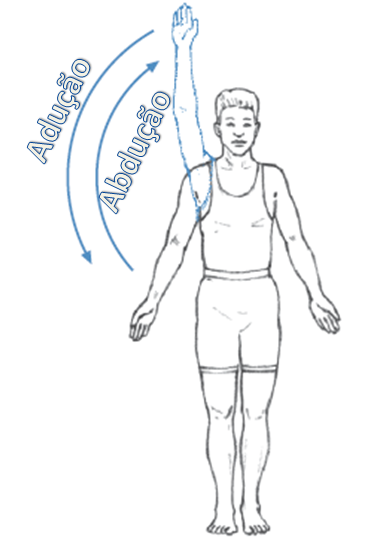
\includegraphics[scale=0.5]{./img/abducao.png}
 % matrixargseg.png: 296x162 pixel, 100dpi, 7.52x4.11 cm, bb=0 0 213 117
 %\caption{Estágio desenvolvimento de jogos ~\cite{fullerton2008game}}
\caption[Movimentos de Abdução e Adução do Braço]{\copyright Movimentos de Abdução e Adução do Braço~\cite{mcginnis2013biomechanics}}
%  \caption{Estágio desenvolvimento de jogos}
 \label{fig:movabducaoaducao}
\end{figure}

Na análise biomecânica do movimento humano, são calculados dois tipos de ângulos:
	\begin{itemize}
		\item Ângulo Relativo: este ângulo é formado entre os eixos longitudinais de segmentos corporais adjacentes~\cite{hamill1999bases}. Logo, os ângulos relativos não descrevem a posição de segmentos ou os lados do ângulo no espaço. Se um indivíduo tem um ângulo relativo de 90º no cotovelo e esse ângulo é mantido, o braço pode ficar em qualquer posição. A interpretação dada a cada segmento irá determinar o tipo de movimento realizado. 
		\item Ângulo Absoluto: este ângulo identifica a orientação angular de um segmento corporal em relação a uma linha fixa de referência~\cite{hamill1999bases}. Dessa forma, os ângulos absolutos devem ser medidos na mesma direção a partir de uma única referência, seja ela horizontal ou vertical.
	\end{itemize}

\section{Máquina de Vetor de Suporte (SVM)}\label{sec:svm_linear}
A teoria da aprendizagem estatística fornece um conjunto de técnicas para a análise de dados, a qual permite a aquisição de conhecimento~\cite{vapnik95}. A máquinas~\ac{svm} faz uso de um conjunto de métodos de aprendizagem supervisionada~\cite{datamining2005} para classificação de dados. Ou seja, a~\ac{svm} é uma ferramenta de predição de classificação, que usa a teoria da aprendizagem de máquina e busca maximizar a acurácia. Normalmente, a~\ac{svm} é aplicada para classificação binária, ou seja, permite classificar os dados em duas classes. No entanto, essa técnica também tem sido aplicada em dados com mais de duas classes~\cite{multisvm2011}.

Um classificador~\ac{svm} foi inicialmente desenvolvido para problemas de aprendizagem linearmente separáveis e utiliza vetores de separação, através de uma técnica de hiperplano de separação ótima ~\cite{vapnik95}. O hiperplano tenta separar as diferentes classes, maximizando a margem entre os pontos extremos de cada classe~\cite{valt2010}. O melhor hiperplano de uma~\ac{svm} é aquele que possui a maior margem entre as duas classes, como pode ser visto na Figura ~\ref{fig:hiperplano}.  

\begin{figure}
 \centering
 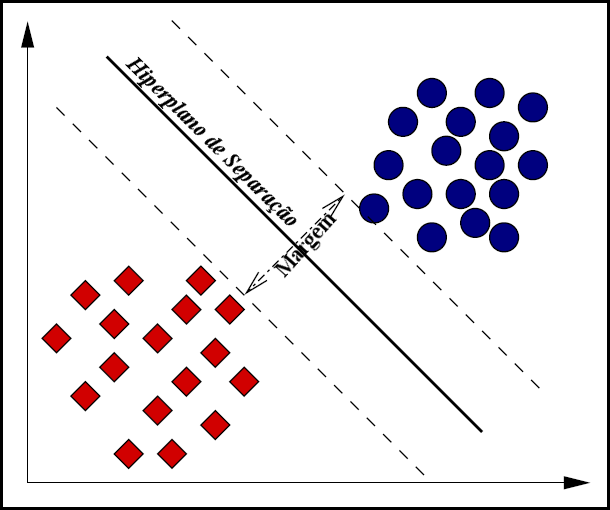
\includegraphics[scale=0.4]{./img/svmhyperplane.png}
 % matrixargseg.png: 296x162 pixel, 100dpi, 7.52x4.11 cm, bb=0 0 213 117
 %\caption{Estágio desenvolvimento de jogos ~\cite{fullerton2008game}}
\caption{Hiperplano de Separação Linear Para Duas Classes}
%  \caption{Estágio desenvolvimento de jogos}
 \label{fig:hiperplano}
\end{figure}


Para entender o funcionamento da ~\ac{svm}, é necessário conhecer a notação:
\begin{math}
R^{n}
\end{math}
é um número real n-dimensional no espaço de vetores. Onde os pontos \textbf{u}, \textbf{v}, \textbf{w} e \textbf{x} serão utilizados para denotar pontos em 
\begin{math}
R^{n}
\end{math}.
Estes pontos são chamados de vetores ou padrões na literatura de Aprendizagem de Máquina.

Cada ponto possui $x_{i}$ e um rótulo $y_{i}$, que denotam a qual classe $x_{i}$ pertence. Logo, se $y_{i} = + 1$, então $x_{i}$ pertence a classe 1; e caso $y_{i} = - 1$, então $x_{i}$ pertence a classe 2. A classificação binária como o nome sugere, significa classificar os dados em duas classes. Para tanto, primeiramente os dados do grupo de treinamento são usados para preencher os espaços com pontos. E depois um segundo grupo de teste é aplicado para verificar a hipótese de qual classe aquele ponto pertence. Formalmente, dado um conjunto de pontos $x_{i}$, qual será os valores $y_{i}$ correspondentes, dado que o classificador possui os padrões adquiridos do grupo de treinamento, além dos rótulos associados a sua classe. A~\ac{svm} irá usar o hiperplano de separação para tentar dividir os dados de treinamento em duas classes. Dessa maneira, o resultado da classificação dos dados de teste dependerá da localização da projeção desses dados.

Formalmente, classificadores que separam os dados por meio de um hiperplano utilizam um discriminante linear~\cite{valt2010} de Equação~\ref{eq:hiperplano}. Um hiperplano é considerado de Margem Máxima (ou de Separação Ótima) quando uma função discriminante consegue separar um conjunto de vetores sem erro. Uma função é discriminante quando consegue discriminar os valores em diferentes padrões. 

O produto escalar $ w.x $ entre os vetores $ w $ e $ x $, $ w $ é o vetor normal ao hiperplano descrito, o vetor \textbf{w} é denominado de peso e a constante parâmetro \textbf{b} é chamada de \textit{bias} ou desvio.
\linebreak
\begin{equation}
f(x)=w^Tx+b=0
\label{eq:hiperplano}
\end{equation}

Se \textbf{u} e \textbf{v} são dois padrões e \textit{f(x)} é a função discriminante, então os valores de \textit{f(\textbf{u})} e \textit{f(\textbf{v})} irão auxiliar na determinação dos valores de \textbf{u} e \textbf{v} que pertencem a classe; logo, a regra para a predição da classe está no Código~\ref{codepredicaoclasse}. 

\begin{lstlisting}[frame=single, caption=Código de Predição da Classes, label=codepredicaoclasse]  % Start your code-block

classificacao = 0;
if (w^t.x + b > = 0)
	classificacao = 1
else
	classificacao = -1;
endif
\end{lstlisting}

A partir desse método de separação de dados lineares, é que a~\ac{svm} foi aplicada para classificar indivíduos diagnosticados com~\ac{dp} ante indivíduos sem o diagnóstico estabelecido. Na Seção~\ref{sec:processador_bio} será explicado como são extraídos os pontos, usando os vetores de características para obtenção da classificação exposta na Seção~\ref{sec:resultado_svm}.

